\chapter{Introduction}
\label{sec:introduction}
\begin{itemize}
\item A vast and connected virtual universe where people can interact, socialize, work, learn and participate in various activities using technology is what is meant by the term "metaversion". This digital world creates a shared, immersive and often three-dimensional space by combining elements of Virtual Reality (VR), Augmented Reality (AR) and the Internet. The word "metaverse" comes from the prefix "meta-" (meaning beyond or beyond) and the word "universe" and refers to an area outside of our physical reality where people can interact, explore, and create their online presence.
\item At the heart of the metaversion are immersive environments that users can explore and interact with through digital avatars. Users can customize these avatars to reflect their identity, tastes and physical characteristics. Metaverse offers a multi-sensory, interactive environment that goes beyond the possibilities of conventional 2D interactions on the Internet and simulates the experience of the real world in a digital environment.
\item In addition to entertainment and social life, metaversion has important implications for work and education. Integrating virtual offices, classrooms and training environments into the metaverse opens up new possibilities for learning, skill development and remote collaboration.
\end{itemize}
\section{History of the Metaverse}
Also known as collective virtual shared space or virtual reality space, the idea of metaversion has a long and evolving history. Science fiction, technology and online communities are its ancestors. Here's a brief overview of the meta version's history:
\subsection{1970 - Sci-Fi Origins:}
The concept of metaversion can be traced back to works of science fiction. Notably, Neal Stephenson's 1992 novel "Snow Crash" introduced the idea of the Metaverse, a virtual reality space where users interacted as avatars. This novel popularized the term and served as a conceptual basis for later developments.
\subsection{Early virtual worlds:}
In the late 1970s and 1980s, online environments such as MUDs (Multi-User Dungeons) and MOOs (MUDs, Object-Oriented) allowed multiple users to interact in text-based virtual worlds. These were the forerunners of modern virtual worlds and online communities.
\subsection{1990 - Emergence of 3D virtual worlds:}
The 1990s saw the emergence of 3D virtual worlds such as Second Life, which allowed users to create avatars, socialize and build their virtual environments. These worlds laid the groundwork for more immersive metaverse experiences.
\subsection{2000 - Online Games and Social Media:}
Online interactions and communities have begun to shape massively multiplayer online games (MMOs) such as World of Warcraft and social media platforms such as Facebook and Twitter, bringing people closer to the idea of connected digital spaces.
\subsection{2010 - VR and AR:}
The development of virtual reality (VR) and augmented reality (AR) technologies has expanded the possibilities of metaversion. Platforms like the Oculus Rift, HTC Vive and the rise of AR via smartphones and AR glasses have begun to make immersive virtual spaces available.
\subsection{Metaverse Investment:}
In the mid-2010s, technology companies began investing heavily in metaversion-related projects. For example, Facebook acquired Oculus VR in 2014 and renamed it Meta in 2021, emphasizing its commitment to building the metaverse.
\subsection{Vision of the Metaverse:}
Companies like Meta (formerly Facebook), Epic Games, and other tech giants have expressed ambitious visions of the metaverse, envisioning a seamless, connected virtual universe where people can work, play, socialize, and engage in various activities.
\subsection{Current developments:}
As of my graduation date in September 2021, various companies are actively developing meta-related technologies such as virtual reality, augmented reality, blockchain, and decentralized platforms. NFTs (Non-Fungible Tokens) have also been used to represent digital assets within the metaverse.
\section{The Future of the Metaverse}
The future of metaversion holds the promise of widespread adoption and integration across various sectors with increasingly immersive virtual and augmented reality experiences, connected virtual worlds, blockchain-based asset ownership, and economic opportunities in digital realms. It will impact society by redefining social dynamics and cultural norms while raising concerns about privacy, security, regulation and environmental sustainability. Artificial intelligence will improve user experience and the metaverse will serve as a platform for education, healthcare, entertainment, gaming, work and collaboration, fundamentally changing the way we interact with the digital realm and each other.
\begin{figure}[h]
    \centering
    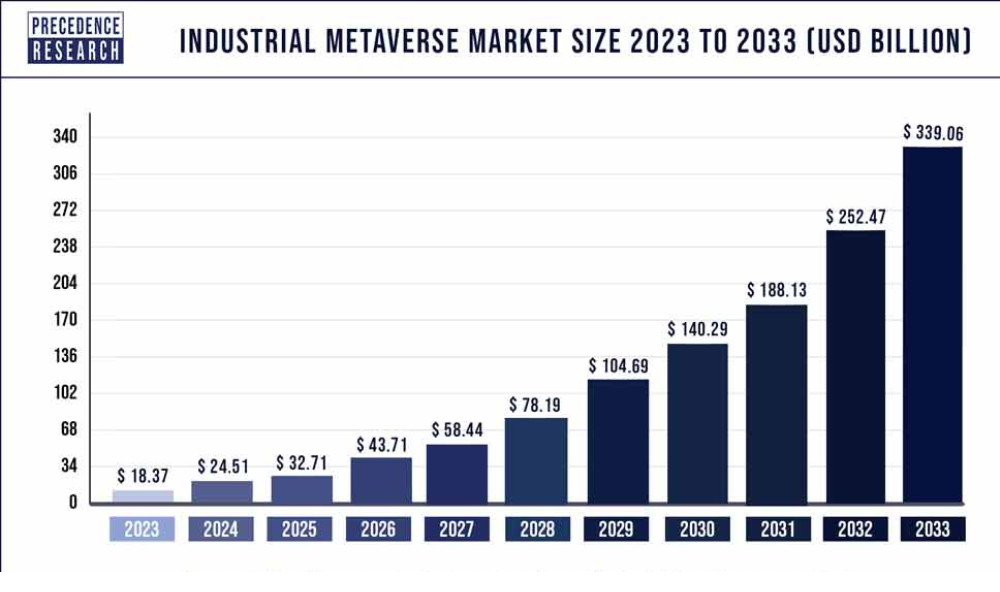
\includegraphics[width=1\linewidth]{Images/industrial-metaverse-market-size.png}
    \caption{Future of Metaverse}
    \label{fig:Future of Metaverse}\cite{metaverse-market}
\end{figure}
\section{How Metaverse Would Excel}
\subsection{What would affect the success of the metaverse}
The success of the metaverse will be influenced by several key factors:\\
\textbf{Technology Advances:}\\ The success of the metaverse depends on the continuous development and advancement of technologies such as virtual reality (VR), augmented reality (AR), blockchain, artificial intelligence (AI), and high-speed internet connectivity. Improved hardware and software are essential to create immersive and seamless virtual experiences.\\
\textbf{User Adoption:}\\ The success of the metaverse depends on a critical mass of users and active participants. The more people get involved and contribute to the metaversion, the more valuable and alive it becomes. User-friendly interfaces and accessibility will play a key role in gaining a diverse user base.\\
\textbf{Content and Creativity:}\\ A wide variety of engaging content, experiences, and activities within the Metaverse is essential. Content creators, developers and users need to be able to easily create and share experiences. This includes virtual worlds, games, social spaces, art, educational content and more.\\
\textbf{Interoperability and standards:}\\ Interoperability between different virtual worlds and platforms is key to a seamless metaverse. Developing open standards and protocols for the metaverse can help create a more connected and accessible environment.\\
\textbf{Security and Privacy:}\\ Users must trust metaverse with their personal data and transactions. Robust security measures, data protection and privacy controls are vital to prevent abuse, fraud and unauthorized access.\\
\textbf{Economic Viability:}\\ A sustainable economy within the metaversion will be necessary to attract users and content creators, including ownership of virtual real estate, digital currencies, and employment opportunities. Blockchain technology and non-fungible tokens (NFTs) can play a role in creating digital property rights and assets.\\
\textbf{Regulation and governance:}\\ Governments and regulators will need to create clear guidelines and legal frameworks for meta